\documentclass[a4paper,11pt]{article}
\usepackage[a4paper,margin=2.5cm]{geometry}
\usepackage[T1]{fontenc}
\usepackage[utf8]{inputenc}
\usepackage[slovak]{babel}
\usepackage{textcomp}
\usepackage{graphicx}
\usepackage[nopatch=item]{microtype}
\usepackage{accsupp}
\graphicspath{{img/}{dokumentacia/img/}}
\setcounter{secnumdepth}{3}
\renewcommand{\thesection}{\arabic{section}.}
\renewcommand{\thesubsection}{\arabic{section}.\arabic{subsection}}
\renewcommand{\thesubsubsection}{\arabic{section}.\arabic{subsection}.\arabic{subsubsection}}
\pagestyle{plain}
\title{SUNS – Zadanie 3: Odhad kalórií z fotografie jedla}
\author{Samuel Bagin}
\date{}
\emergencystretch=2em

\input{glyphtounicode}
\pdfgentounicode=1
\DeclareUnicodeCharacter{00B2}{\BeginAccSupp{method=hex,unicode,ActualText=00B2}\texttwosuperior\EndAccSupp{}}

\newcommand{\screenshot}[2]{%
  \begin{minipage}[c]{#1\linewidth}
  \centering
  \includegraphics[width=\linewidth,keepaspectratio]{#2}
  \end{minipage}}
\newcommand{\images}[1]{%
  \begin{center}
  #1%
  \end{center}}
\newcommand{\notebookoutput}[1]{%
  \par\begingroup\small\ttfamily\raggedright\setlength{\parskip}{0pt}#1\par\endgroup}

\begin{document}
\maketitle

\section{Analýza, párovanie a rozdelenie dát}

% main.ipynb — bunka 2
\subsection{Audit a párovanie obrázkov s metadátami}

V \texttt{metadata.csv} je \texttt{file\_name} relatívna cesta k snímke, \texttt{id} identifikátor taniera a \texttt{total\_calories} cieľ v kcal. Stĺpec \texttt{total\_mass} uvádza hmotnosť v gramoch a \texttt{total\_fat}, \texttt{total\_carb} a \texttt{total\_protein} uvádzajú množstvá makroživín. Zoznam ingrediencií je v \texttt{metadata.json}. Každá ingrediencia má \texttt{id}, \texttt{name}, \texttt{grams}, \texttt{calories}, \texttt{fat}, \texttt{carb} a \texttt{protein}.

Párovanie podľa \texttt{file\_name} overuje prítomnosť práve jedného obrázka a jedného záznamu. Pri pripájaní ingrediencií kontrolujeme aj \texttt{id}. Audit pôvodného behu našiel 3 260 RGB snímok s rozlíšením 640 × 480, bez duplicitných identifikátorov a bez chýbajúcich hodnôt v CSV.

% main.ipynb — bunka 3
\images{\screenshot{0.267}{audit-pocty.png}%
  \hspace{0.012\linewidth}%
  \screenshot{0.235}{audit-rozlisenie.png}%
  \hspace{0.012\linewidth}%
  \screenshot{0.245}{audit-chybajuce-hodnoty.png}}

% main.ipynb — bunka 4
Najvyššia anotovaná hodnota (3 943,3 kcal) patrí snímke \texttt{dish\_1560974769}. V zázname je 2 991 g ryže, čo podľa snímky pôsobí ako nadhodnotená gramáž. Záznam patrí do trénovacej množiny a ponechávame ho v pôvodnej podobe. Jeho vplyv pri trénovaní preveruje konfigurácia CNN s Huberovou stratou (Malé chyby penalizuje kvadraticky, veľké chyby lineárne. Vďaka tomu majú odľahlé hodnoty pri trénovaní menší vplyv než pri kvadratickej strate (MSE).).

% main.ipynb — bunka 5
\subsection{Trénovacia, validačná a testovacia množina}

Snímky so zhodnými pixelmi alebo s rovnakou kombináciou ingrediencií a gramáží ostávajú v jednej množine. Pri skupinovom rozdelení stratifikujeme podľa kalorických kvantilov. Priemer a smerodajnú odchýlku cieľa na jeho štandardizáciu počítame z tréningu. V pôvodnom behu malo rozdelenie 2 328 trénovacích, 466 validačných a 466 testovacích obrázkov.

% main.ipynb — bunka 6
\images{\screenshot{0.41}{rozdelenie-statistika.png}%
  \hspace{0.012\linewidth}%
  \screenshot{0.578}{rozdelenie-kalorie.png}}
\notebookoutput{
  Jedinečné skupiny: 3029
}

% main.ipynb — bunka 7
\section{CNN}

\subsection{Generátory dát}

Generátor načíta RGB obrázky v dávkach po 64, zmenší ich na 96 × 96 pixelov, prevedie intenzity do intervalu od 0 do 1 a normalizuje kanály konštantami ImageNetu. Trénovacie dávky sa miešajú a snímky prechádzajú rotáciou a zrkadlením (augmentácia). Validácia a test používajú pevné poradie bez augmentácie. Pri výpočte tréningových metrík používame takisto pevné poradie a snímky bez augmentácie.

% main.ipynb — bunka 8
\images{\screenshot{0.76}{generator-ukazky.png}}
\notebookoutput{
  Vstup batchu: (64, 3, 96, 96) \textbar{} cieľ: (64,)
}

% main.ipynb — bunka 9
\subsection{Trénovanie}

\subsubsection{Návrh siete a konfigurácie hyperparametrov}

CNN má tri bloky s konvolúciou 3 × 3, BatchNorm, ReLU a poolingom. Regresná hlava používa dropout. Tréning využíva aj augmentáciu a weight decay v optimalizátore AdamW.

\textbf{Tok základnej konfigurácie C1.} Rozmery máp sú výška × šírka × kanály. Každý konvolučný filter spracúva všetky vstupné kanály a vytvorí jednu mapu príznakov. Jadrá majú priestorový rozmer 3 × 3. Krok 1 a padding 1 zachovávajú výšku aj šírku. MaxPool vezme maximum z každého okna 2 × 2 a zmenší oba priestorové rozmery na polovicu.

% ```mermaid
% flowchart TB
%     image[["RGB vstup po normalizácii<br/>96 × 96 × 3"]]
% 
%     subgraph block1["Blok 1 · 16 filtrov"]
%         direction LR
%         conv1["Conv2d<br/>jadrá 3 × 3 × 3"] --> act1["BatchNorm → ReLU"]
%         act1 --> maps1[["96 × 96 × 16"]]
%         maps1 --> pool1["MaxPool 2 × 2"]
%         pool1 --> out1[["48 × 48 × 16"]]
%     end
% 
%     subgraph block2["Blok 2 · 32 filtrov"]
%         direction LR
%         conv2["Conv2d<br/>jadrá 3 × 3 × 16"] --> act2["BatchNorm → ReLU"]
%         act2 --> maps2[["48 × 48 × 32"]]
%         maps2 --> pool2["MaxPool 2 × 2"]
%         pool2 --> out2[["24 × 24 × 32"]]
%     end
% 
%     subgraph block3["Blok 3 · 64 filtrov"]
%         direction LR
%         conv3["Conv2d<br/>jadrá 3 × 3 × 32"] --> act3["BatchNorm → ReLU"]
%         act3 --> maps3[["24 × 24 × 64"]]
%         maps3 --> pool3["MaxPool 2 × 2"]
%         pool3 --> out3[["12 × 12 × 64"]]
%     end
% 
%     subgraph head["Regresná hlava CNN"]
%         direction LR
%         avg["AdaptiveAvgPool<br/>3 × 3 × 64"] --> flat["Flatten<br/>576 hodnôt"]
%         flat --> hidden["Linear 576 → 96<br/>ReLU → Dropout 0,25"]
%         hidden --> prediction["Linear 96 → 1<br/>štandardizovaný odhad"]
%     end
% 
%     image --> block1 --> block2 --> block3 --> head
%     head --> kcal["Spätná škála<br/>1 odhad v kcal"]
% 
%     classDef tensor fill:#440154,stroke:#440154,color:#ffffff;
%     classDef convolution fill:#3b528b,stroke:#3b528b,color:#ffffff;
%     classDef pooling fill:#21918c,stroke:#126662,color:#071f20;
%     classDef dense fill:#5ec962,stroke:#318342,color:#102912;
%     classDef result fill:#fde725,stroke:#8c7912,color:#2b2400;
%     class image,maps1,out1,maps2,out2,maps3,out3 tensor;
%     class conv1,act1,conv2,act2,conv3,act3 convolution;
%     class pool1,pool2,pool3,avg pooling;
%     class flat,hidden,prediction dense;
%     class kcal result;
% ```
\images{\screenshot{0.675}{cnn-architektura.png}}
\images{\screenshot{1}{cnn-architektura-detail.pdf}}
Základ \textbf{C1} má šírku 16, dropout 0,25, krok učenia 0,001, weight decay 0,0001 a stratu MSE. Ďalšie konfigurácie menia po jednom faktore: \textbf{C2} znižuje krok na 0,0003, \textbf{C3} zvyšuje dropout na 0,45, \textbf{C4} zväčšuje šírku na 24, \textbf{C5} zvyšuje weight decay na 0,01 a \textbf{C6} používa Huberovu stratu s hranicou 0,5 v štandardizovanej škále.

% main.ipynb — bunka 11
\subsubsection{Priebeh trénovania a vyhodnotenie}

Checkpoint vyberáme podľa validačnej MAE. Ak víťaz dosiahne najlepší checkpoint v posledných 18 epochách základného behu, pokračuje najviac do 150 epoch. Graf ukazuje validačný priebeh všetkých konfigurácií a porovnanie trénovacej a validačnej krivky víťaza.

Vo výsledkových tabuľkách je \textbf{Ep.} epocha zvoleného checkpointu, MSE je v kcal², MAE a RMSE sú v kcal a R² je bezrozmerné. Tučným písmom je označený model vybraný podľa validačného pravidla popísaného pri danej skupine.

\images{\screenshot{0.81}{cnn-trenovanie.png}}

% main.ipynb — bunka 14
\images{\screenshot{0.77}{cnn-vysledky.png}}

% main.ipynb — bunka 15
\images{\screenshot{0.68}{cnn-rezidua.png}}

% main.ipynb — bunka 16
V pôvodnom behu vyhrala \textbf{C1}. Po úvodných výkyvoch sa tréningová aj validačná krivka ustálili bez postupného rozchádzania. Chyba bola výrazne menšia než pri predikovaní tréningového priemeru, takže výsledok nevykazoval výrazné podtrénovanie ani pretrénovanie vybraného checkpointu. Kladný reziduál znamená podhodnotenie energie.

C1 dosiahla MAE 65,7 kcal na tréningu a 76,9 kcal na teste. Pri kalorickejších jedlách majú testové reziduály väčší rozptyl a model viaceré z nich podhodnocuje. Tréningový extrém s anotáciou okolo 3 943 kcal prispel k vyššiemu RMSE na tréningu (116,1 kcal) než na teste (108,5 kcal).

\section{Zhlukovanie pomocou transfer learningu}

Transfer learning prenáša reprezentácie naučené na zdrojovej úlohe do novej úlohy. MobileNetV3 Small bol predtrénovaný na klasifikáciu obrázkov v ImageNete. Tu jeho pevné váhy využijeme na extrakciu tvarov, textúr a ďalších obrazových príznakov. Tieto príznaky poslúžia na zhlukovanie aj na trénovanie kalorických regresorov.

\subsection{MobileNet}

MobileNetV3 Small má 2 542 856 parametrov. Po nahradení klasifikátora identitou zostáva 927 008 zmrazených parametrov. Transformácie ImageNetu použijú stredový výrez 224 × 224 a normalizujú kanály. V \texttt{features\_df} má každý z 576 príznakov vlastný stĺpec. Dva ďalšie stĺpce obsahujú \texttt{file\_name} a \texttt{total\_calories}.

% ```mermaid
% flowchart LR
%     image["RGB snímka"] --> prep["ImageNet transformácie: výrez 224 × 224"]
%     prep --> mobile["Zmrazený MobileNetV3 Small bez klasifikátora"]
%     mobile --> embedding["576 obrazových príznakov"]
%     embedding --> cluster["L2 normalizácia → PCA → K-means"]
%     embedding --> regress["MLP, SVR alebo ExtraTrees"]
%     regress --> kcal["Odhad v kcal"]
% ```
\images{\screenshot{1}{mobilenet-architektura.png}}

% main.ipynb — bunka 17
\notebookoutput{
  MobileNet: 2,542,856 parametrov; extraktor: 927,008\\
  Rozmery tabuľky príznakov: (3260, 578)
}

% main.ipynb — bunka 18
\subsection{Zhlukovanie príznakov}

\subsubsection{Algoritmus a výber počtu zhlukov}

Obrazové vektory L2 normalizujeme, PCA ich zmenší na 50 rozmerov a K-means vytvorí zhluky. Počet zhlukov od 2 do 8 vyberáme podľa najvyššieho silhouette skóre (Porovnáva priemernú vzdialenosť bodu od ostatných bodov vo vlastnom zhluku s priemernou vzdialenosťou od bodov v najbližšom inom zhluku). Cestu k snímke, kalórie a ingrediencie používame až pri interpretácii.

$$
\scriptstyle
s(i)=\frac{b(i)-a(i)}{\max\{a(i),b(i)\}}
\qquad
S=\frac{1}{n}\sum\limits_{i=1}^{n}s(i)
\qquad
\begin{array}{l}
\scriptscriptstyle a(i)\;\mbox{\tiny - priemerná vzdialenosť od ostatných bodov v rovnakom clusteri} \\
\scriptscriptstyle b(i)\;\mbox{\tiny - najmenšia priemerná vzdialenosť od ostatných bodov z iných clusterov}
\end{array}
$$

% main.ipynb — bunka 19
\images{\screenshot{0.26}{zhluky-statistika.png}%
  \hspace{0.012\linewidth}%
  \screenshot{0.728}{zhluky-vyber.png}}
\notebookoutput{
  PCA zachovaná variancia: 0.815 \textbar{} počet zhlukov: 2
}

% main.ipynb — bunka 20
\subsubsection{Ukážky fotografií a priemerné obrázky}

Každý riadok zobrazuje tri obrázky najbližšie k centroidu, tri náhodné príklady a priemerný RGB obrázok zo všetkých snímok daného zhluku.

% main.ipynb — bunka 21
\images{\screenshot{1}{zhluky-fotografie.png}}

% main.ipynb — bunka 22
Priemerný obrázok zhluku vznikne spriemerovaním všetkých fotiek v danom zhluku. Fotky sa najprv zmenšia na 96 × 96 pixelov. Potom sa na každej pozícii zvlášť spriemeruje červená, zelená a modrá zložka zo všetkých fotiek. V zhluku 0 vidno väčšiu farebnú plochu uprostred. V zhluku 1 zostáva viac svetlej plochy taniera, čo zodpovedá menším porciám na ukážkach.

% main.ipynb — bunka 23
\subsubsection{Analýza výsledkov zhlukovania}

V pôvodnom behu boli vybrané dva zhluky so silhouette 0,160. Ide o široké skupiny s čiastočne sa prekrývajúcim vzhľadom.

Zhluk 0 (priemer 336,13 kcal) zahŕňa najmä plnšie taniere s kombináciami mäsa, zeleniny a príloh. Na priemernom obrázku vidno väčšiu hnedozelenú plochu v strede. V zhluku 1 (priemer 141,35 kcal) sa častejšie objavujú menšie porcie, napríklad kúsky zemiakov alebo ovocia. Na priemernom obrázku je menšia plocha jedla a viac viditeľného taniera. Rozdiel priemerov je približne 195 kcal. K zoskupeniu prispieva plocha jedla aj kompozícia záberu.

\section{Trénovanie regresorov na extrahovaných príznakoch}

Regresory používajú rovnakých 576 príznakov MobileNetu. MLP a SVR sa učia nad škálovanými príznakmi a predikujú štandardizovaný cieľ, ktorý následne prevedieme do kcal (odhad v kcal = výstup modelu × smerodajná odchýlka kcal + priemer kcal). ExtraTrees používa priamo hodnoty príznakov a kalórie. Parametre škálovania sa počítajú z trénovacej množiny.

\subsection{Transfer – MLP}

Pred MLP StandardScaler štandardizuje každý zo 576 príznakov zvlášť. Sieť ich spracuje cez vrstvy 576 → 128 → 32 → 1. Tréning používa LayerNorm, dropout a predčasné zastavenie podľa validačnej MAE.

% ```mermaid
% flowchart LR
%     embedding["576 príznakov MobileNetu"] --> scale["Tréningový StandardScaler"]
%     scale --> hidden["Husté vrstvy 128 a 32"]
%     hidden --> output["Lineárny výstup"]
%     output --> kcal["Spätná škála: odhad v kcal"]
% ```
\images{\screenshot{0.94}{mlp-architektura.png}}


% main.ipynb — bunka 25
\images{\screenshot{0.46}{mlp-trenovanie.png}\hspace{0.012\linewidth}%
  \screenshot{0.528}{mlp-vysledky.png}}

% main.ipynb — bunka 26
MLP dosiahla MAE 27,3 kcal na tréningu a 60,0 kcal na teste. Rast validačného RMSE pri klesajúcej tréningovej chybe naznačuje pretrénovanie. MLP mala najnižšiu validačnú MAE spomedzi kandidátov s obrazovými príznakmi, ale jej validačná RMSE bola vyššia než pri CNN.

\subsection{SVR a ExtraTrees}

SVR používa RBF jadro a skúša štyri hodnoty penalizácie \texttt{C}. ExtraTrees kombinuje 400 stromov a skúša tri minimálne veľkosti listu. Tieto modely sa netrénujú po epochách.

% ```mermaid
% flowchart LR
%     embedding["576 príznakov MobileNetu"] --> scaler["Tréningový StandardScaler"]
%     scaler --> svr["SVR s RBF jadrom"]
%     svr --> inverse["Spätný prevod do kcal"]
%     embedding --> trees["ExtraTrees: priemer predikcií stromov"]
%     inverse --> kcal["Odhad v kcal"]
%     trees --> kcal
% ```
\images{\screenshot{0.98}{svr-extratrees-architektura.png}}
Finálny regresor vyberáme spomedzi kandidátov vrátane MLP. Kandidát musí na validácii zlepšiť MAE aj RMSE vybranej CNN. Spomedzi takých kandidátov vyberáme najnižšiu validačnú MAE. Tabuľka zobrazuje validačné R² podľa formátu výsledkov.

% main.ipynb — bunka 28
\images{\screenshot{0.705}{regresory-vysledky.png}}

% main.ipynb — bunka 29
Validačné MAE a RMSE boli 72,6 a 105,4 kcal pri CNN C1, 67,1 a 103,6 kcal pri SVR C=1, a 68,2 a 101,0 kcal pri SVR C=10. Obe konfigurácie SVR zlepšili obe metriky CNN. O výbere C=1 rozhodla nižšia validačná MAE. Jeho testová MAE 61,2 kcal bola o 20,5 \% nižšia než pri CNN.

\section{Bonus}

\subsection{Zobrazenie filtrov z konvolučných vrstiev - BONUS}

Prvá vrstva má RGB vstupy, preto farby jadra vyjadrujú váhy troch farebných kanálov. Napríklad filter 8 v pôvodnom behu zachytáva pásový farebný kontrast a filter 9 rozdiel medzi stredom a okolím. V hlbších vrstvách farby označujú vybrané naučené kanály. Aktivačné mapy ukazujú odozvu na konkrétnu snímku, od jemnejších hrán a textúr až po hrubšie obrazové štruktúry.

% main.ipynb — bunka 30
\images{\screenshot{0.494}{cnn-filtre-prva-vrstva.png}%
  \hspace{0.012\linewidth}%
  \screenshot{0.494}{cnn-filtre-hlbsie-vrstvy.png}}
\images{\screenshot{0.89}{cnn-aktivacne-mapy.png}}

% main.ipynb — bunka 31
\subsection{Regresia pomocou Transformera - BONUS}

\subsubsection{Vstup a architektúra ViT}

TinyViT sa učí z RGB obrázkov od začiatku. Snímku 96 × 96 rozdelí na 36 výrezov s veľkosťou 16 × 16. Každý výrez mapuje na 64-rozmerný token a pridá token CLS a pozičné príznaky. Tri bloky so štyrmi hlavami self-attention premiešajú informácie medzi tokenmi. Regresná hlava číta výstupný token CLS.

CLS (\textit{classification token}) je naučiteľný 64-rozmerný vektor, ktorý model pridáva na začiatok sekvencie pred 36 tokenov z obrazových výrezov. Na začiatku tréningu je inicializovaný nulami. V každom bloku získava cez self-attention informácie z celej sekvencie. Po treťom bloku regresná hlava z výsledného CLS vypočíta štandardizovaný odhad, ktorý sa následne prevedie na kcal. Obrázok~\ref{fig:tinyvit-tok} zobrazuje tok dát a rozmery tokenov v jednotlivých častiach modelu.

% ```mermaid
% flowchart LR
%     image["Normalizované RGB 96 × 96"] --> patches["36 výrezov 16 × 16"]
%     patches --> tokens["Projekcia na 64 prvkov, pozície a CLS"]
%     tokens --> transformer["3 bloky, každý so 4 hlavami self-attention"]
%     transformer --> head["Výstup CLS → regresná hlava"]
%     head --> kcal["Spätná škála: odhad v kcal"]
% ```
\begin{center}
  \begin{minipage}{\linewidth}
    \centering
    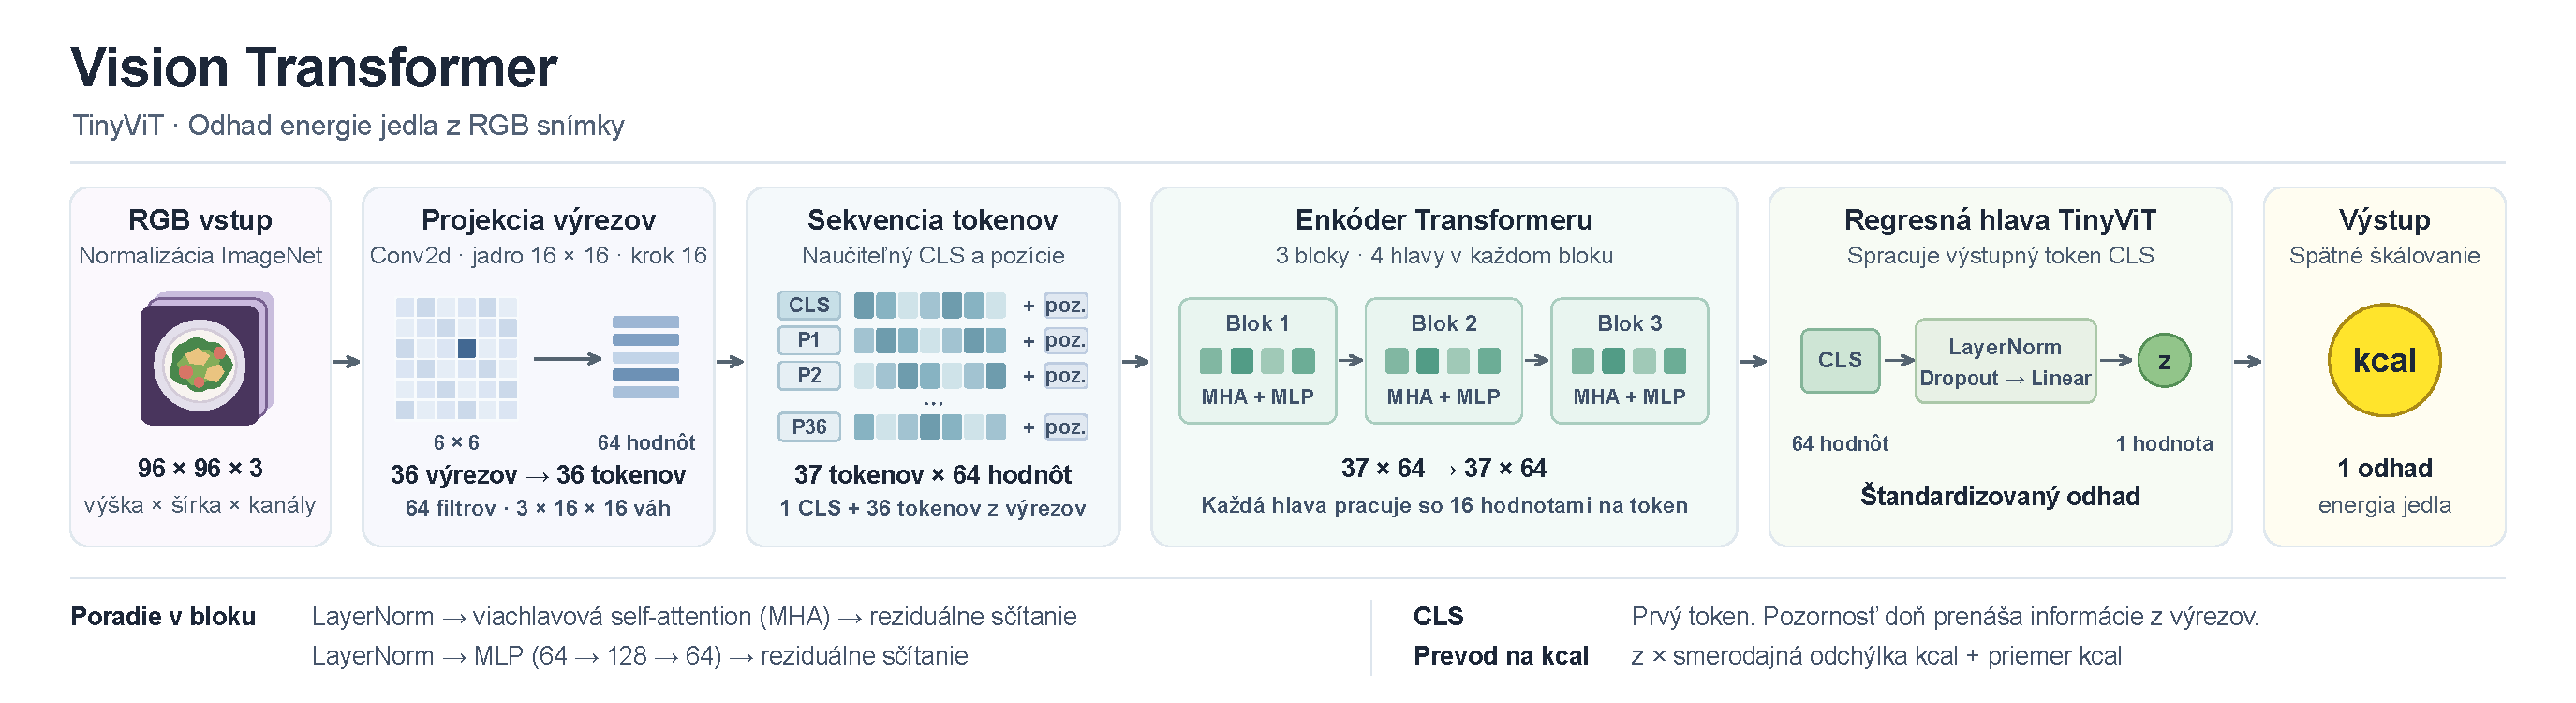
\includegraphics[width=\linewidth]{vit-architektura.pdf}\par\smallskip
    \refstepcounter{figure}\label{fig:tinyvit-tok}
  \end{minipage}
\end{center}

% main.ipynb — bunka 32
\notebookoutput{
  Počet parametrov TinyViT: 152257
}

% main.ipynb — bunka 33
\subsubsection{Priebeh trénovania a vyhodnotenie}

Mapa pozornosti ukazuje, ako posledná vrstva prerozdelila pozornosť z CLS na obrazové výrezy validačnej snímky. Ide o priemer cez štyri hlavy.

% main.ipynb — bunka 34
\images{\screenshot{0.46}{vit-trenovanie.png}\hspace{0.012\linewidth}%
  \screenshot{0.528}{vit-vysledky.png}}

% main.ipynb — bunka 35
\images{\screenshot{0.81}{vit-mapa-pozornosti.png}}

% main.ipynb — bunka 36
V pôvodnom behu vybral validačný postup checkpoint z epochy 74. TinyViT dosiahol testovú MAE 87,3 kcal a R² 0,635. Jeho chyba bola vyššia než pri CNN (76,9 kcal) aj pri vybranom SVR (61,2 kcal).

\end{document}
